\chapter{\label{lesson16}Пропорциональный регулятор}
{\bfseries Анонс:}\\\\
Датчик освещенности. Соревнования «Линия». Особенности движения по линии. Пропорциональный регулятор. Калибровка.\\\\
{\bfseries Цели:}
\begin{itemize}
	\item{}{\bfseries Обучающие:} Познакомить учащихся с режимами работы датчика освещенности. Закрепить принципы релейного регулирования. Изучить пропорциональный регулятор.
	\item{}{\bfseries Развивающая:} Обеспечить развитие навыков анализа своей деятельности и творческого мышления.\\
\end{itemize}	
{\bfseries Ход занятия:}\\\\
\begin{tabular}[h!]{lll}
	{\hyperlink{lesson16x1}{1. Организационный момент}}&{Презентация}&{(5 мин)}\\
	{\hyperlink{lesson16x2}{2. Соревнования «Линия»}}&{Игра}&{(40 мин)}\\
	{\hyperlink{lesson16x3}{3. Анализ технических решений}}&{Рефлексия}&{(10 мин)}\\
	{\hyperlink{lesson16x4}{4. Пропорциональный регулятор}}&{Презентация}&{(10 мин)}\\
	{\hyperlink{lesson16x5}{5. Проблемы калибровки}}&{Презентация}&{(15 мин)}\\
\end{tabular}\\\\

{\hypertarget{lesson16x1}{\blackBlueText{I. Организационный момент}}}\\\\		
\clearpage
{\hypertarget{lesson16x2}{\blackBlueText{II. Соревнования «Линия»}}}\\\\	

Для выполнения следующего задания нам понадобиться датчик освещенности. При инициализации датчика цвета на выбор предлагается 4 режима. В силу некоторых физических причин \greenText{каких?} , если датчик цвета предполагается использовать в режиме освещенности, оптимально выбирать подсветку именно красным цветом, т.е. режим Lego Color-Red.

\begin{figure}[h!]
	\begin{center}
		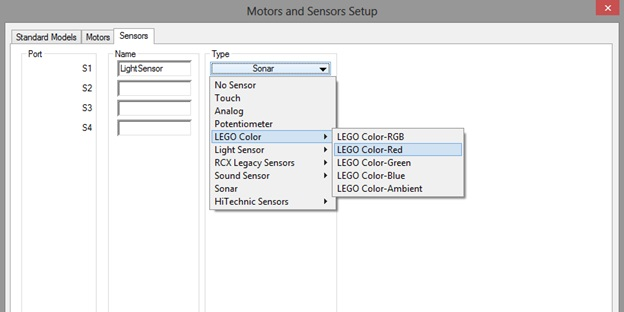
\includegraphics[width=1\linewidth]{chapters/chapter16/images/1}
		\caption{}
		\label{ris:image16x1}
	\end{center}
\end{figure}	

Уровень освещенности  измеряется в условных единицах. Используя написанную программу тестирования датчика (занятие~\ref{lesson12}) можно предложить учащимся определить значения освещенности для черного и белого цветов на поле.

{\slshape Следующее соревнование позволяет повторить передаточные соотношения и релейный регулятор. Соревнования лучше сделать командными, команда~--- 2--3 человека.}\\\\

Регламент соревнований:
\begin{enumerate}
	\item За наиболее короткое время робот, следуя черной линии, должен добраться от места старта до места финиша.
	\item {\bfseries Если робот потеряет линию более чем на 5 секунд, он будет дисквалифицирован.} (Покидание линии, при котором никакая часть робота не находится над линией, может быть допустимо только по касательной и не должно быть больше чем три длины корпуса робота. Длина робота в этом случае считается по колесной базе.)
	\item  Во время проведения состязания участники команд не должны касаться роботов.
	\item  Команде дается не менее двух попыток. В зачет идет лучшее время.
	\item  Победителем будет объявлена команда, потратившая на преодоление дистанции наименьшее время.\\\\
\end{enumerate}

{\hypertarget{lesson16x3}{\blackBlueText{III. Анализ технических решений}}}\\\\	

Конструкция тележки очень схожа с подобной для движения вдоль стенки с тем только отличием, что вместо датчика расстояния, повернутого горизонтально влево, используется датчик освещенности/цвета, «смотрящий» вниз. Поэтому будем пользоваться конструкцией тележки из раздела «движение вдоль стенки». Датчик собирает информацию из некоторого телесного угла (то есть с площади круга на поверхности, на которую «смотрит» датчик, причем эта площадь тем больше, чем больше расстояние от датчика до поверхности).

\begin{figure}[h!]
	\begin{center}
		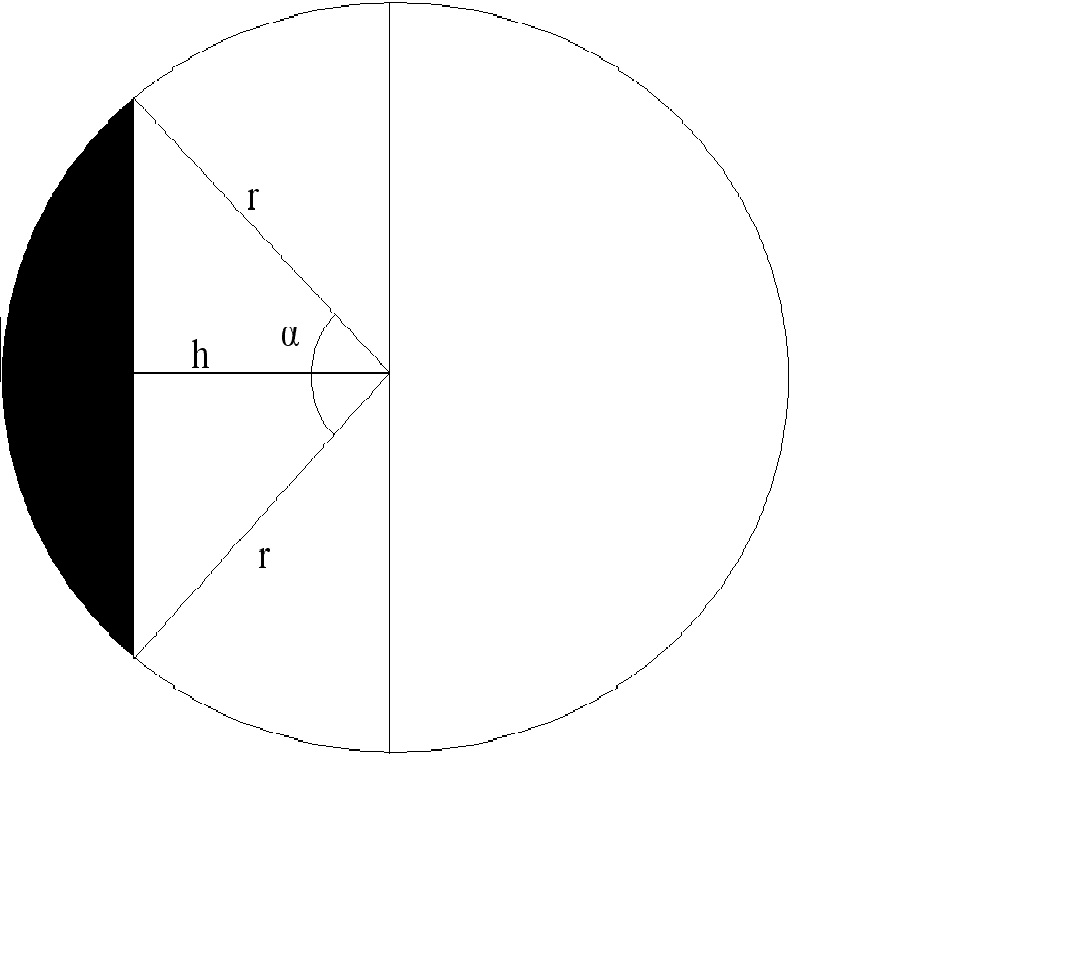
\includegraphics[width=0.5\linewidth]{chapters/chapter16/images/2}
		\caption{Так датчик освещенности «видит» линию.}
		\label{ris:image16x2}
	\end{center}
\end{figure}

В зависимости от соотношения черного и белого в круге, который «видит» робот показания датчика освещенности будут меняться. Понятно, что при различных смещениях робота относительно линии картина будет меняться. Для того, что бы решить задачу управления необходимо, что бы зависимость между смещением тележки и показаниями датчика была монотонной. Оказывается это возможно не при всех соотношениях между \(D\) (шириной линии) и \(r\) (радиусом круга видимости). 

\begin{figure}[h!]
	\begin{center}
		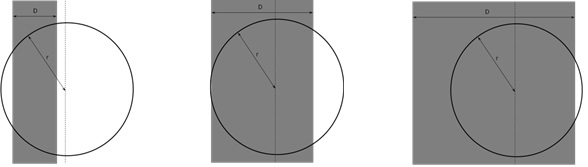
\includegraphics[width=0.79\linewidth]{chapters/chapter16/images/3}
		\caption{Как датчик освещенности «видит» линии разной толщины.}
		\label{ris:image16x3}
	\end{center}
\end{figure}

При \(D<r\) задачу управления решить не удастся, так как не будет наблюдаться монотонной зависимости между смещением \(h\) и показаниями датчика. 

При \(r<D<2r\) показания датчика освещенности не достигнут максимального аппаратного значения (все поле черное). С точки зрения управления, допустимыми являются отклонения вплоть до того, как \(h=h_{max}=D–r\). При больших отклонениях управляемая система не поймет, что датчик находится с другой стороны линии, и будет выполнять действия, противоположные правильным. В последнем случае (\(D>2r\)) максимальное показание датчика будет равно 1. Этот вариант также подходит для движения вдоль границы черной и белой полуплоскостей.

В большинстве случаев разумным является размещение датчика освещенности на высоте 1--2 см над поверхностью. Тогда радиус круга, с поверхности которого датчик регистрирует сигнал, оказывается равным 0,5--1,0 см. Редко встречаются задачи, в которых ширина линии оказывается меньше 2--3 см, так что почти всегда можно полагать, что \(D>2r\).

Реализация релейного регулятора в данном случае может выглядеть так, где param~--- значение датчика освещенности, соответствующее среднему положению (полкруга белое, полкруга черное):\\\\

{\programm
	{\slshape\bC{while}}\rC{(\bC{\slshape true})}\\
	\rC{\{}\\
	\indent{\slshape\bC{if}}\rC{(\bbC{SensorValue}[\rrC{LightSensor}] > \rrC{param})}\\
	\indent\rC{\{}\\
	\indent\indent\bbC{motor}\rC{[\rrC{motorB}] =  \rrC{100};}\\
	\indent\indent\bbC{motor}\rC{[\rrC{motorC}] =  \rrC{50};}\\
	\indent\rC{\}}\\
	\indent{\slshape\bC{else}}\\
	\indent\rC{\{}\\
	\indent\indent\bbC{motor}\rC{[\rrC{motorB}] =  \rrC{50};}\\
	\indent\indent\bbC{motor}\rC{[\rrC{motorC}] =  \rrC{100};}\\
	\indent\rC{\}}\\
	\indent\bbC{wait1Msec}\rC{(\rrC{1});}\\
	\rC{\}}\\
}\\\\

Стремясь к победе в гонках учащиеся, скорее всего, максимально увеличивали мощность, подаваемую на моторы, и собирали повышающую передачу. Эти казалось бы разумные действия приводили к массовым вылетам с трассы, так что скорее всего победителем оказался не самый быстрый робот, но тот который смог пройти всю трассу. Однако можно увеличить скорость движения робота по линии, изменив алгоритм управления на пропорциональный регулятор.\\\\

{\hypertarget{lesson16x4}{\blackBlueText{IV. Пропорциональный регулятор}}}\\\\

Пропорциональный регулятор~--- тип обратной связи, при котором на управляемый элемент подается сигнал, пропорциональный значению сигнала от датчика. То есть, например, чем больше сигнал от датчика, тем больше (или меньше) сигнал, подаваемый на управляемую систему. Логику пропорционального регулятора можно проиллюстрировать следующим абстрактным примером: Если сигнал от датчика освещенности обозначим переменной lum, то на мотор будем подавать мощность k*lum (k~--- некоторый постоянный заранее заданный коэффициент). Параметр k из рассмотренного примера называют коэффициентом усиления пропорционального регулятора. Как видно из примера, чем больше показания датчика, тем быстрее (если k>0) будет крутиться мотор. То есть чем ярче свет, который видит робот, тем быстрее он будет к нему двигаться. С точки зрения программирования пропорциональный регулятор чаще всего описывается следующей блок схемой:

\begin{figure}[h!]
	\begin{center}
		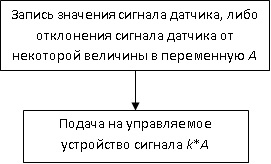
\includegraphics[width=0.75\linewidth]{chapters/chapter16/images/4}
		\caption{}
		\label{ris:image16x4}
	\end{center}
\end{figure}

Теперь учащимся следует дать возможность реализовать пропорциональный регулятор самостоятельно, на тех же конструкциях, что и в начале занятия.\\\\
Реализация пропорционального регулятора:\\\\

{\programm
	{\slshape\bC{while}}\rC{(\bC{\slshape true})}\\
	\rC{\{}\\
	\indent up \rC{=} k \rC{* (}S1 \rC{- } param\rC{);}\\
	\indent\bbC{motor}\rC{[\rrC{motorB}] =  \rrC{50} \rC{+}} up\rC{;}\\
	\indent\bbC{motor}\rC{[\rrC{motorB}] =  \rrC{50} \rC{-}} up\rC{;}\\
	\rC{\}}\\
}\\\\

где S1~--- текущее значение освещенности, а param~--- желаемое.\\\\

{\hypertarget{lesson16x5}{\blackBlueText{V. Проблемы калибровки}}}\\\\

С использованием пропорционального регулятора роботы стали меньше вихлять и значительно ускорились. Однако, стоит выключить в классе свет~--- и они сходят с дистанции. Проблему можно решить, подобрав новое значение param, к которому мы стремимся. Однако, значение средней освещенности, подобранное в классе, может не совпасть с условиями освещенности на соревнованиях и робот не сможет ехать по линии. Да и на самих соревнованиях между попытками проходит довольно много времени и освещенность меняется. 

Каков вообще смысл этого среднего значения освещенности param, которое мы подбирали? Как уже было сказано, робот еде по границе черного и белого. Логично, что  его идеальное положение, к которому регулятор направляет его, должно быть таким: полкруга видимости робота белые, полкруга~--- черные.\\\\

\greenText{Рис.}\\\\

В если робот знает значения White (белый при данном освещении) и Black ( черный при данном освещении), то значение param=(White+Black)/2 , может быть вычислено программно. Остается найти способ сообщать роботу значения черного и белого перед каждой попыткой.  Реализаций существует множество.

{\slshape Следует дать детям возможность самостоятельно придумать алгоритмы реализации калибровки, на следующем занятии у них будет возможность их опробовать.}